\documentclass[12pt,a4paper,UTF8]{article}
\usepackage{ctex} % Chinese support
\usepackage{graphicx} % Insert images
\usepackage{subfigure}
\usepackage{float}
\usepackage{listings} % Print source code
\usepackage{color} % Color support
\usepackage{booktabs} % Professional table support
\usepackage{pdflscape} % Landscape pages support in PDF
\usepackage{hyperref} % Hypertext links support for cross-referencing
\usepackage{amsmath,mathtools}
\usepackage{ulem} % strikethrough
\usepackage{diagbox} % diagonal in tabular


% Customize hyperref format (it's set to no special format here)
\hypersetup{hidelinks}

% Declare directories to search for graphics files for graphicx
\graphicspath{{figures/}}

% Define source code style for listings
\lstdefinestyle{verilog-style}{
	language=Verilog,
	basicstyle=\ttfamily\footnotesize,
	keywordstyle=\bfseries\color[rgb]{0, 0, 1},
	identifierstyle=\color[rgb]{0.5, 0.3, 0.1},
	stringstyle=\color[rgb]{0.6, 0.1, 0.1},
	commentstyle=\itshape\color[rgb]{0.05, 0.5, 0.05},
	backgroundcolor=\color[gray]{0.95},
	numbers=left,
	numbersep=5pt,
	numberstyle=\color[gray]{0.6},
	breaklines=true
}

\newcommand{\reporttitle}[2]{
  \LARGE\textsf{#1}\quad\underline{\makebox[12em]{#2}}
}

\newcommand{\reportinfo}[2]{
  \large\makebox[4em]{\textsf{#1}}\quad\underline{\makebox[18em]{#2}}
}

\begin{document}
\begin{titlepage}
  \centering
  \vspace*{\fill}
  {\Huge\textsf{数字电路与数字系统实验}} \\ [100pt]
  \reportinfo{实验名称}{exp02 译码器和编码器} \\ [10pt]
  \reportinfo{院系}{计算机科学与技术系} \\ [10pt]
  \reportinfo{学生姓名}{} \\ [10pt]
  \reportinfo{学号}{} \\ [10pt]
  \reportinfo{班级}{数字电路与数字系统实验1班} \\ [10pt]
  \reportinfo{邮箱}{} \\ [10pt]
  \reportinfo{实验时间}{2020 年 9 月 16 日} \\ [10pt]
  \vspace*{\fill}
\end{titlepage}
\tableofcontents
\newpage

\section{实验目的}
\begin{itemize}
  \item 复习译码器和编码器的相关知识
  \item 学习Verilog的for循环
  \item 理解并实现优先编码器
  \item 学会操作DE10-Standard开发板上的数码管
  \item \sout{少写亿点bug}
\end{itemize}

\section{实验原理}
\begin{description}
  \item[\hspace{2em}\textsf{译码器}] 输入$n$位二进制编码,输出$2^n$中取1码
  \item[\hspace{2em}\textsf{编码器}] 译码器的反函数电路
  \item[\hspace{2em}\textsf{七段数码管}] 每一段都对应输入的一个最小项之和或最大项之积
  \item[\hspace{2em}\textsf{优先编码器}] 如果出现多个输入同时有效,输出按输入优先级编码
\end{description}

\section{实验环境/器材}
\begin{itemize}
  \item Quartus编辑器和DE10-Standard开发平台
  \item FPGA开发板
\end{itemize}

\section{程序代码 + 实验步骤/过程 + 测试方法}
\subsection{实验2.2.2 优先编码器}
这是一个高位优先的优先级编码器,所以当使能有效时,输入依次从低位到高位逐个由0变成1即可
\begin{lstlisting}[style=verilog-style]
	en = 0; x = 4'b0000; #10;
	x[0] = 1; #10;
	x[1] = 1; #10;
	x[2] = 1; #10;
	x[3] = 1; #10;
	
	en = 1; x = 4'b0000; #10;
	x[0] = 1; #10;
	x[1] = 1; #10;
	x[2] = 1; #10;
	x[3] = 1; #10;
\end{lstlisting}

\begin{figure}[H]
  \centering
  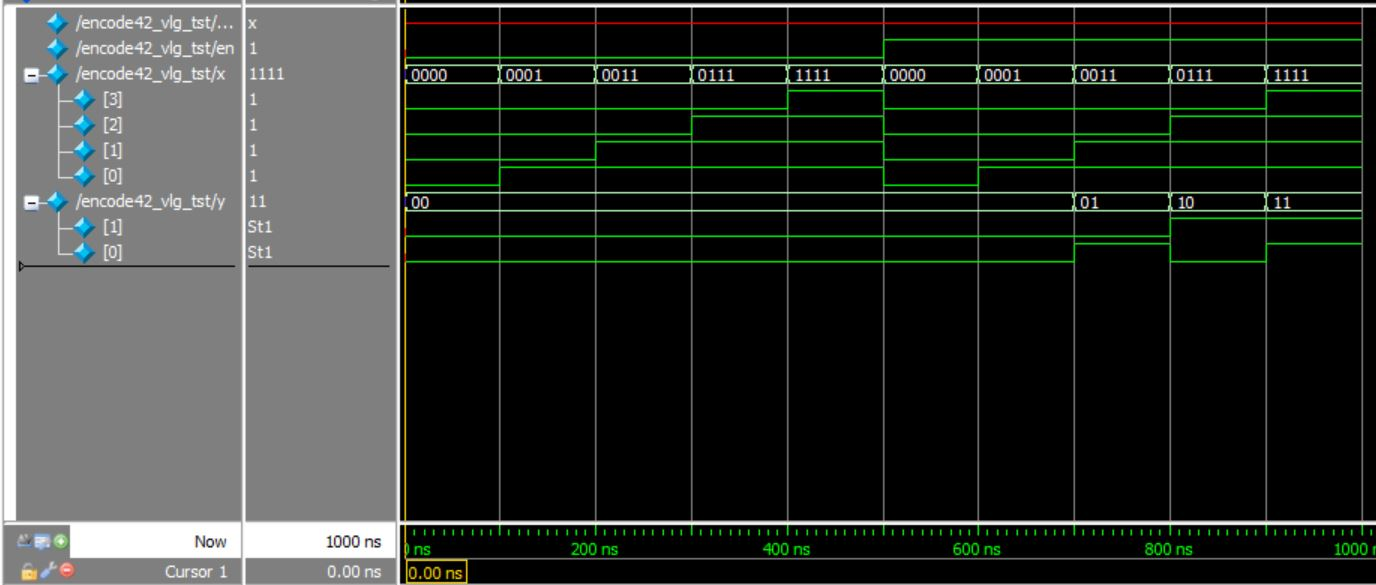
\includegraphics[width=0.8\textwidth]{2_2_2sim.JPG}
  \caption{运行仿真结果}
  \label{encoder_sim}
\end{figure}

\subsection{实验2.2.3 七段数码管}
先根据真值表画一下分别七个LED的卡诺图 \\
\hspace*{2em}\sout{可以用logisim偷懒(输入真值表自动生成卡诺图和表达式)} \\
\begin{figure}[H]
  \centering
  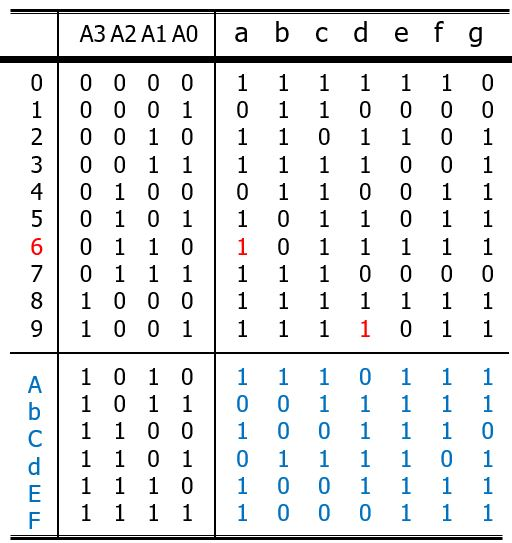
\includegraphics[width=0.8\textwidth]{truth_table_7seg.JPG}
  \caption{七段译码器真值表}
  \label{truth_table_7seg}
\end{figure}

注意该真值表中1表示该段LED有效,对应的Y[i]应为0,
所以用该真值表对应的卡诺图化简的结果均为Y[i]' \\

{\noindent$\left.
  \begin{tabular}[H]{|r|c|c|c|c|}
    \hline
    \diagbox{X3X2}{X1X0} & 00 & 01 & 11 & 10 \\ \hline
    00                   & 1  & 0  & 1  & 1  \\ \hline
    01                   & 0  & 1  & 1  & 1  \\ \hline
    11                   & 1  & 0  & 1  & 1  \\ \hline
    10                   & 1  & 1  & 0  & 1  \\ \hline
  \end{tabular}
  \right.$ \\ \\
$Y0' = (X3 + X2 + X1 + X0') (X3 + X2' + X1 + X0) %
  (X3' + X2 + X1' + X0') (X3' + X2' + X1 + X0')$
\\ \\
$\left.
  \begin{tabular}[H]{|r|c|c|c|c|}
    \hline
    \diagbox{X3X2}{X1X0} & 00 & 01 & 11 & 10 \\ \hline
    00                   & 1  & 1  & 1  & 1  \\ \hline
    01                   & 1  & 0  & 1  & 0  \\ \hline
    11                   & 0  & 1  & 0  & 0  \\ \hline
    10                   & 1  & 1  & 0  & 1  \\ \hline
  \end{tabular}
  \right.$\\ \\
$Y1' = (X3 + X2' + X1 + X0') (X2' + X1' + X0)%
  (X3' + X1' + X0') (X3' + X2' + X0)$
\\ \\
$\left.
  \begin{tabular}[H]{|r|c|c|c|c|}
    \hline
    \diagbox{X3X2}{X1X0} & 00 & 01 & 11 & 10 \\ \hline
    00                   & 1  & 1  & 1  & 0  \\ \hline
    01                   & 1  & 1  & 1  & 1  \\ \hline
    11                   & 0  & 1  & 0  & 0  \\ \hline
    10                   & 1  & 1  & 1  & 1  \\ \hline
  \end{tabular}
  \right.$\\ \\
$Y2' = (X3 + X2 + X1' + X0) (X3' + X2' + X0) (X3' + X2' + X1')$
\\ \\
$\left.
  \begin{tabular}[H]{|r|c|c|c|c|}
    \hline
    \diagbox{X3X2}{X1X0} & 00 & 01 & 11 & 10 \\ \hline
    00                   & 1  & 0  & 1  & 1  \\ \hline
    01                   & 0  & 1  & 0  & 1  \\ \hline
    11                   & 1  & 1  & 0  & 1  \\ \hline
    10                   & 1  & 1  & 1  & 0  \\ \hline
  \end{tabular}
  \right.$\\ \\
$Y3' = (X3 + X2 + X1 + X0') (X3 + X2' + X1 + X0)%
  (X2' + X1' + X0') (X3' + X2 + X1' + X0)$
\\ \\
$\left.
  \begin{tabular}[H]{|r|c|c|c|c|}
    \hline
    \diagbox{X3X2}{X1X0} & 00 & 01 & 11 & 10 \\ \hline
    00                   & 1  & 0  & 0  & 1  \\ \hline
    01                   & 0  & 0  & 0  & 1  \\ \hline
    11                   & 1  & 1  & 1  & 1  \\ \hline
    10                   & 1  & 0  & 1  & 1  \\ \hline
  \end{tabular}
  \right.$\\ \\
$Y4' = (X3 + X0') (X2 + X1 + X0') (X3 + X2' + X1)$
\\ \\
$\left.
  \begin{tabular}[H]{|r|c|c|c|c|}
    \hline
    \diagbox{X3X2}{X1X0} & 00 & 01 & 11 & 10 \\ \hline
    00                   & 1  & 0  & 0  & 0  \\ \hline
    01                   & 1  & 1  & 0  & 1  \\ \hline
    11                   & 1  & 0  & 1  & 1  \\ \hline
    10                   & 1  & 1  & 1  & 1  \\ \hline
  \end{tabular}
  \right.$\\ \\
$Y5' = (X3 + X2 + X0') (X3 + X2 + X1') %
  (X3 + X1' + X0') (X3' + X2' + X1 + X0')$
\\ \\
$\left.
  \begin{tabular}[H]{|r|c|c|c|c|}
    \hline
    \diagbox{X3X2}{X1X0} & 00 & 01 & 11 & 10 \\ \hline
    00                   & 0  & 0  & 1  & 1  \\ \hline
    01                   & 1  & 1  & 0  & 1  \\ \hline
    11                   & 0  & 1  & 1  & 1  \\ \hline
    10                   & 1  & 1  & 1  & 1  \\ \hline
  \end{tabular}
  \right.$\\ \\
$Y6' = (X3 + X2 + X1) (X3 + X2' + X1' + X0') (X3' + X2' + X1 + X0)$
\\ \\
}

在Quartus中实现:
\begin{lstlisting}[style=verilog-style]
	assign Y[0] = (X[3] & X[2] & X[1] & ~X[0]) | (X[3] & ~X[2] & X[1] & X[0]) | (~X[3] & X[2] & ~X[1] & ~X[0]) | (~X[3] & ~X[2] & X[1] & ~X[0]);
	assign Y[1] = (X[3] & ~X[2] & X[1] & ~X[0]) | (~X[2] & ~X[1] & X[0]) | (~X[3] & ~X[1] & ~X[0]) | (~X[3] & ~X[2] & X[0]);
	assign Y[2] = (X[3] & X[2] & ~X[1] & X[0]) | (~X[3] & ~X[2] & X[0]) | (~X[3] & ~X[2] & ~X[1]);
	assign Y[3] = (X[3] & X[2] & X[1] & ~X[0]) | (X[3] & ~X[2] & X[1] & X[0]) | (~X[2] & ~X[1] & ~X[0]) | (~X[3] & X[2] & ~X[1] & X[0]);
	assign Y[4] = (X[3] & ~X[0]) | (X[2] & X[1] & ~X[0]) | (X[3] & ~X[2] & X[1]);
	assign Y[5] = (X[3] & X[2] & ~X[0]) | (X[3] & X[2] & ~X[1]) | (X[3] & ~X[1] & ~X[0]) | (~X[3] & ~X[2] & X[1] & ~X[0]);
	assign Y[6] = (X[3] & X[2] & X[1]) | (X[3] & ~X[2] & ~X[1] & ~X[0]) | (~X[3] & ~X[2] & X[1] & X[0]);
\end{lstlisting}

\begin{figure}[H]
  \centering
  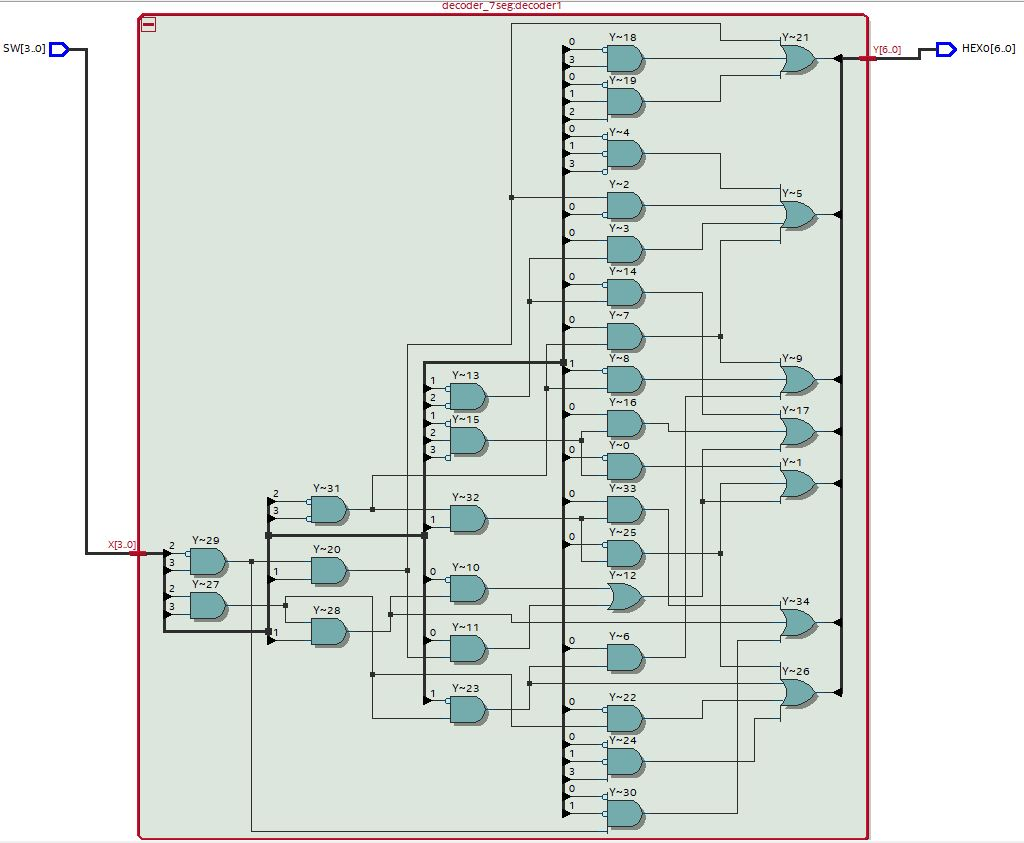
\includegraphics[width=0.8\textwidth]{2_2_3RTL.JPG}
  \caption{RTL Viewer}
  \label{7seg_RTL}
\end{figure}
\hspace*{\fill} \\

下载到FPGA开发板上验证,满足实验要求
\begin{figure}[H]
  \centering
  \subfigure{
    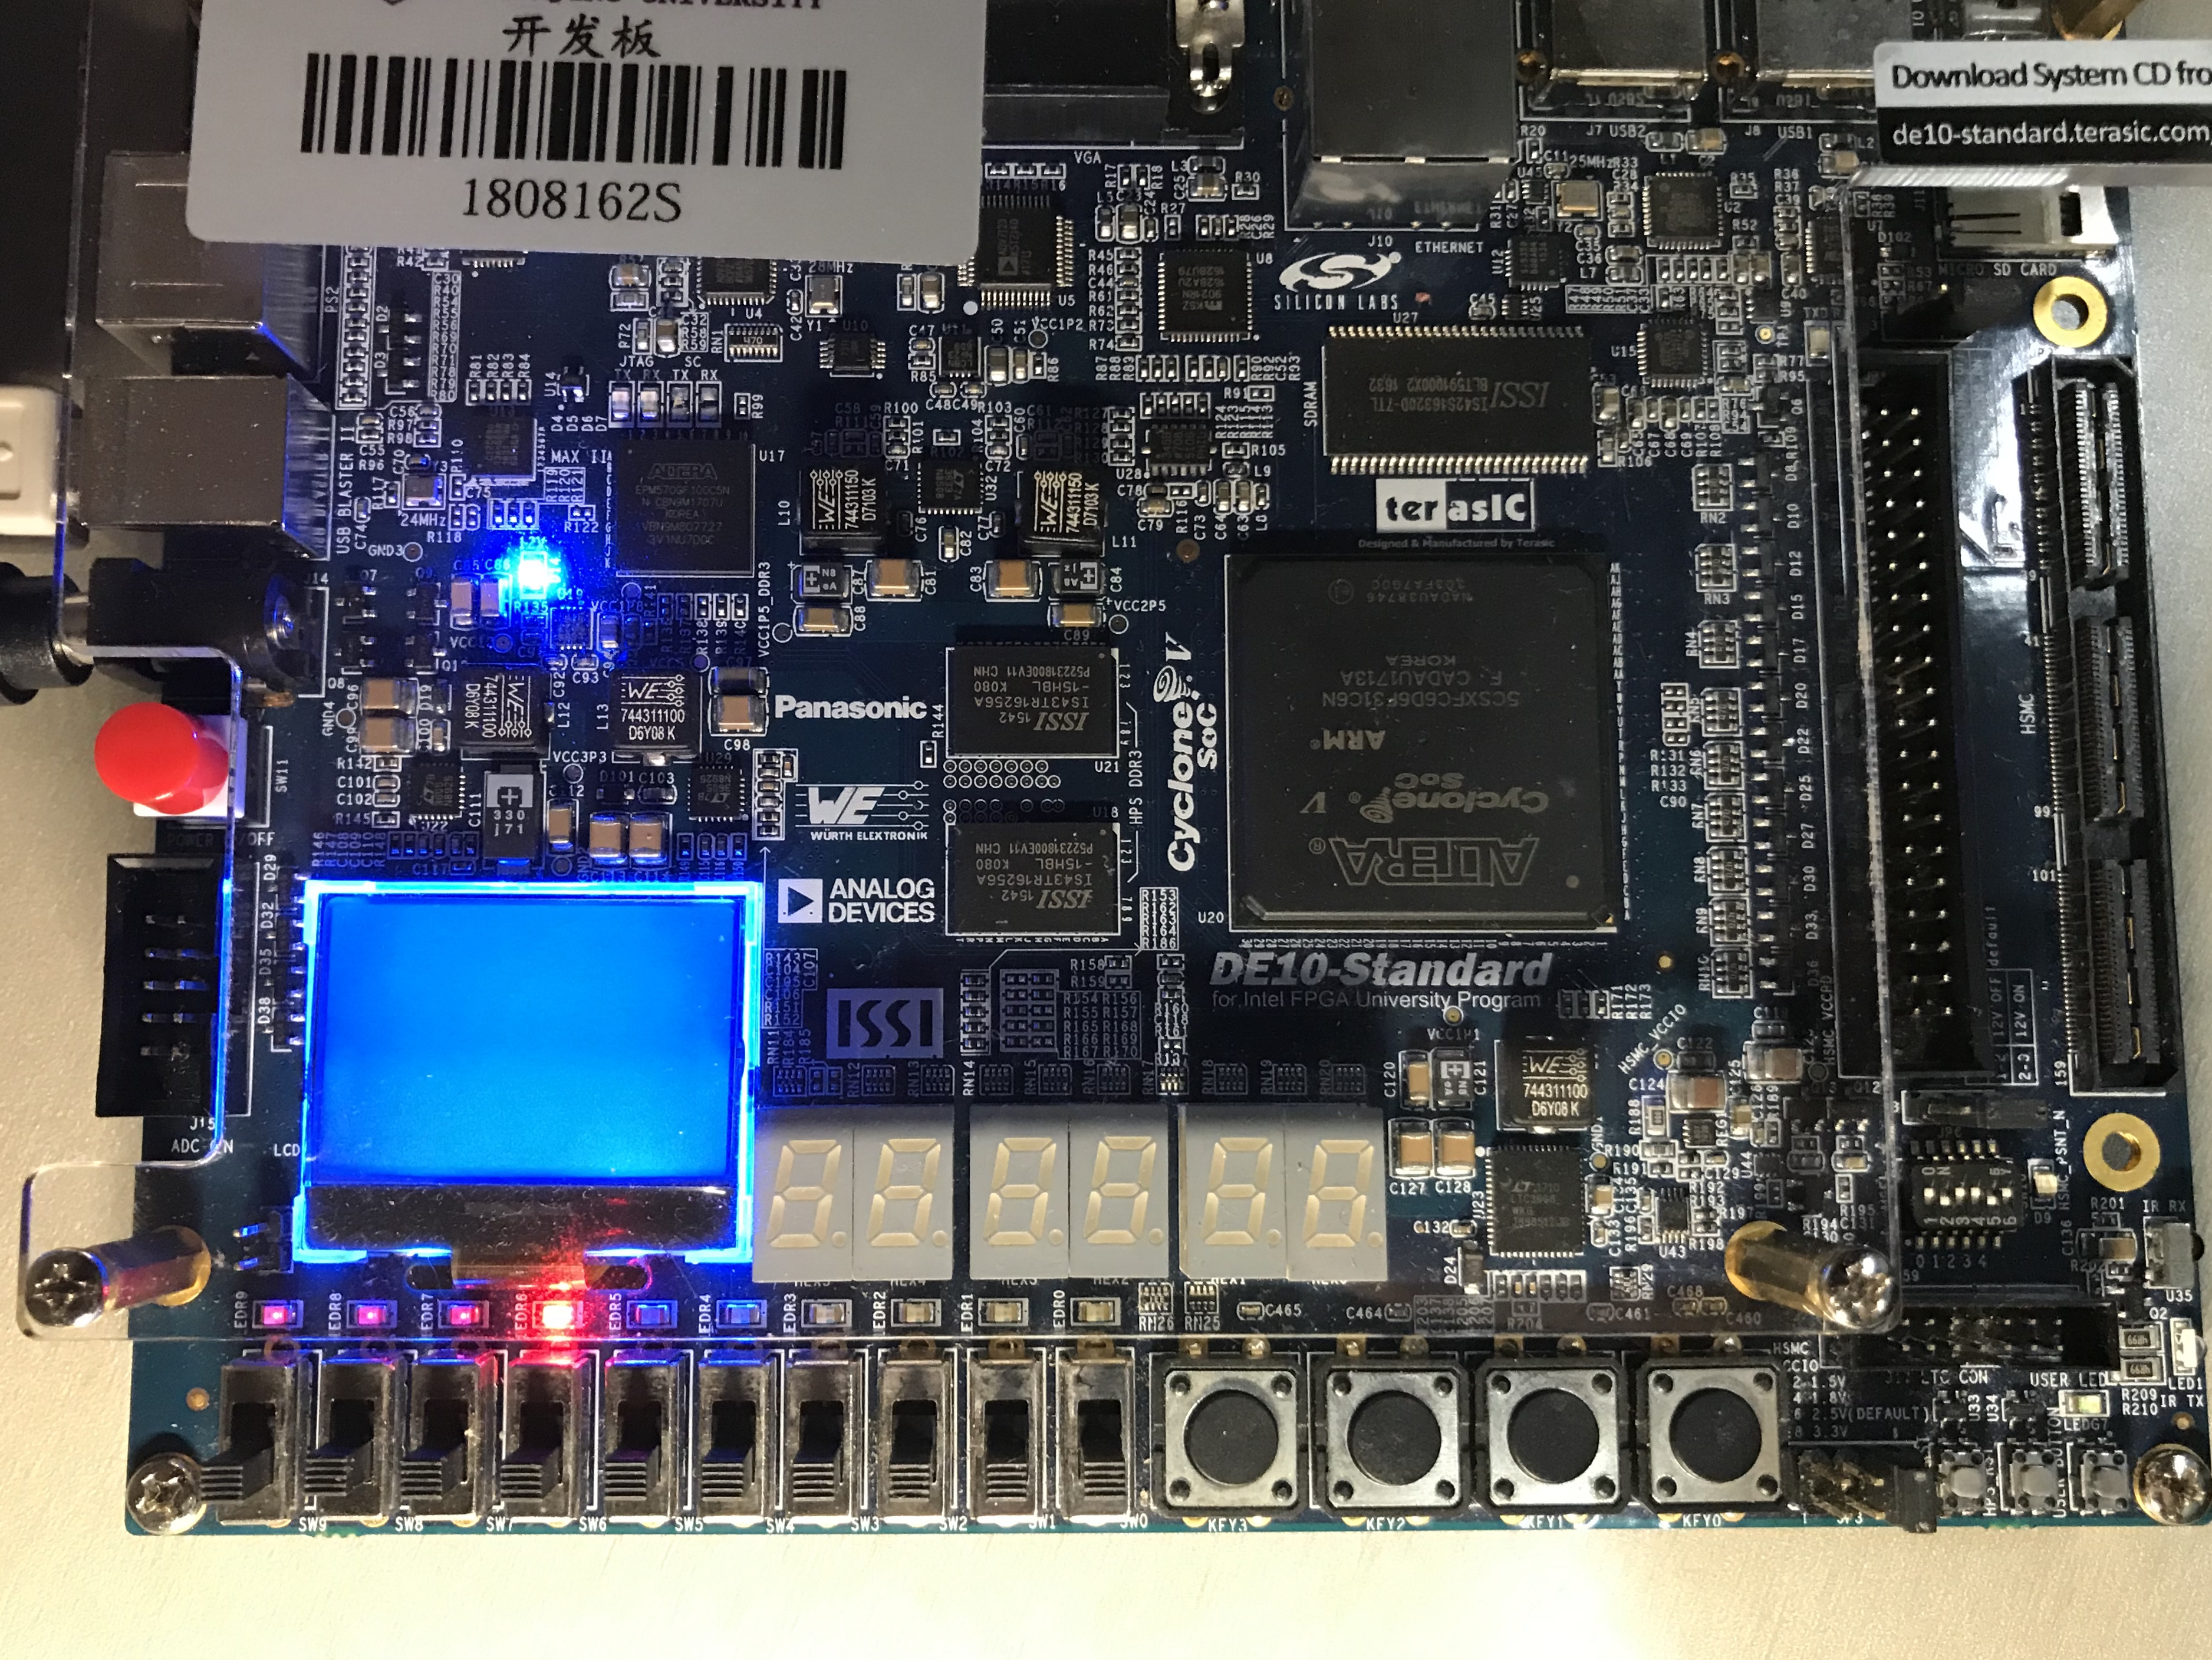
\includegraphics[width=0.45\textwidth]{fpga1.JPG}
  }
  \subfigure{
    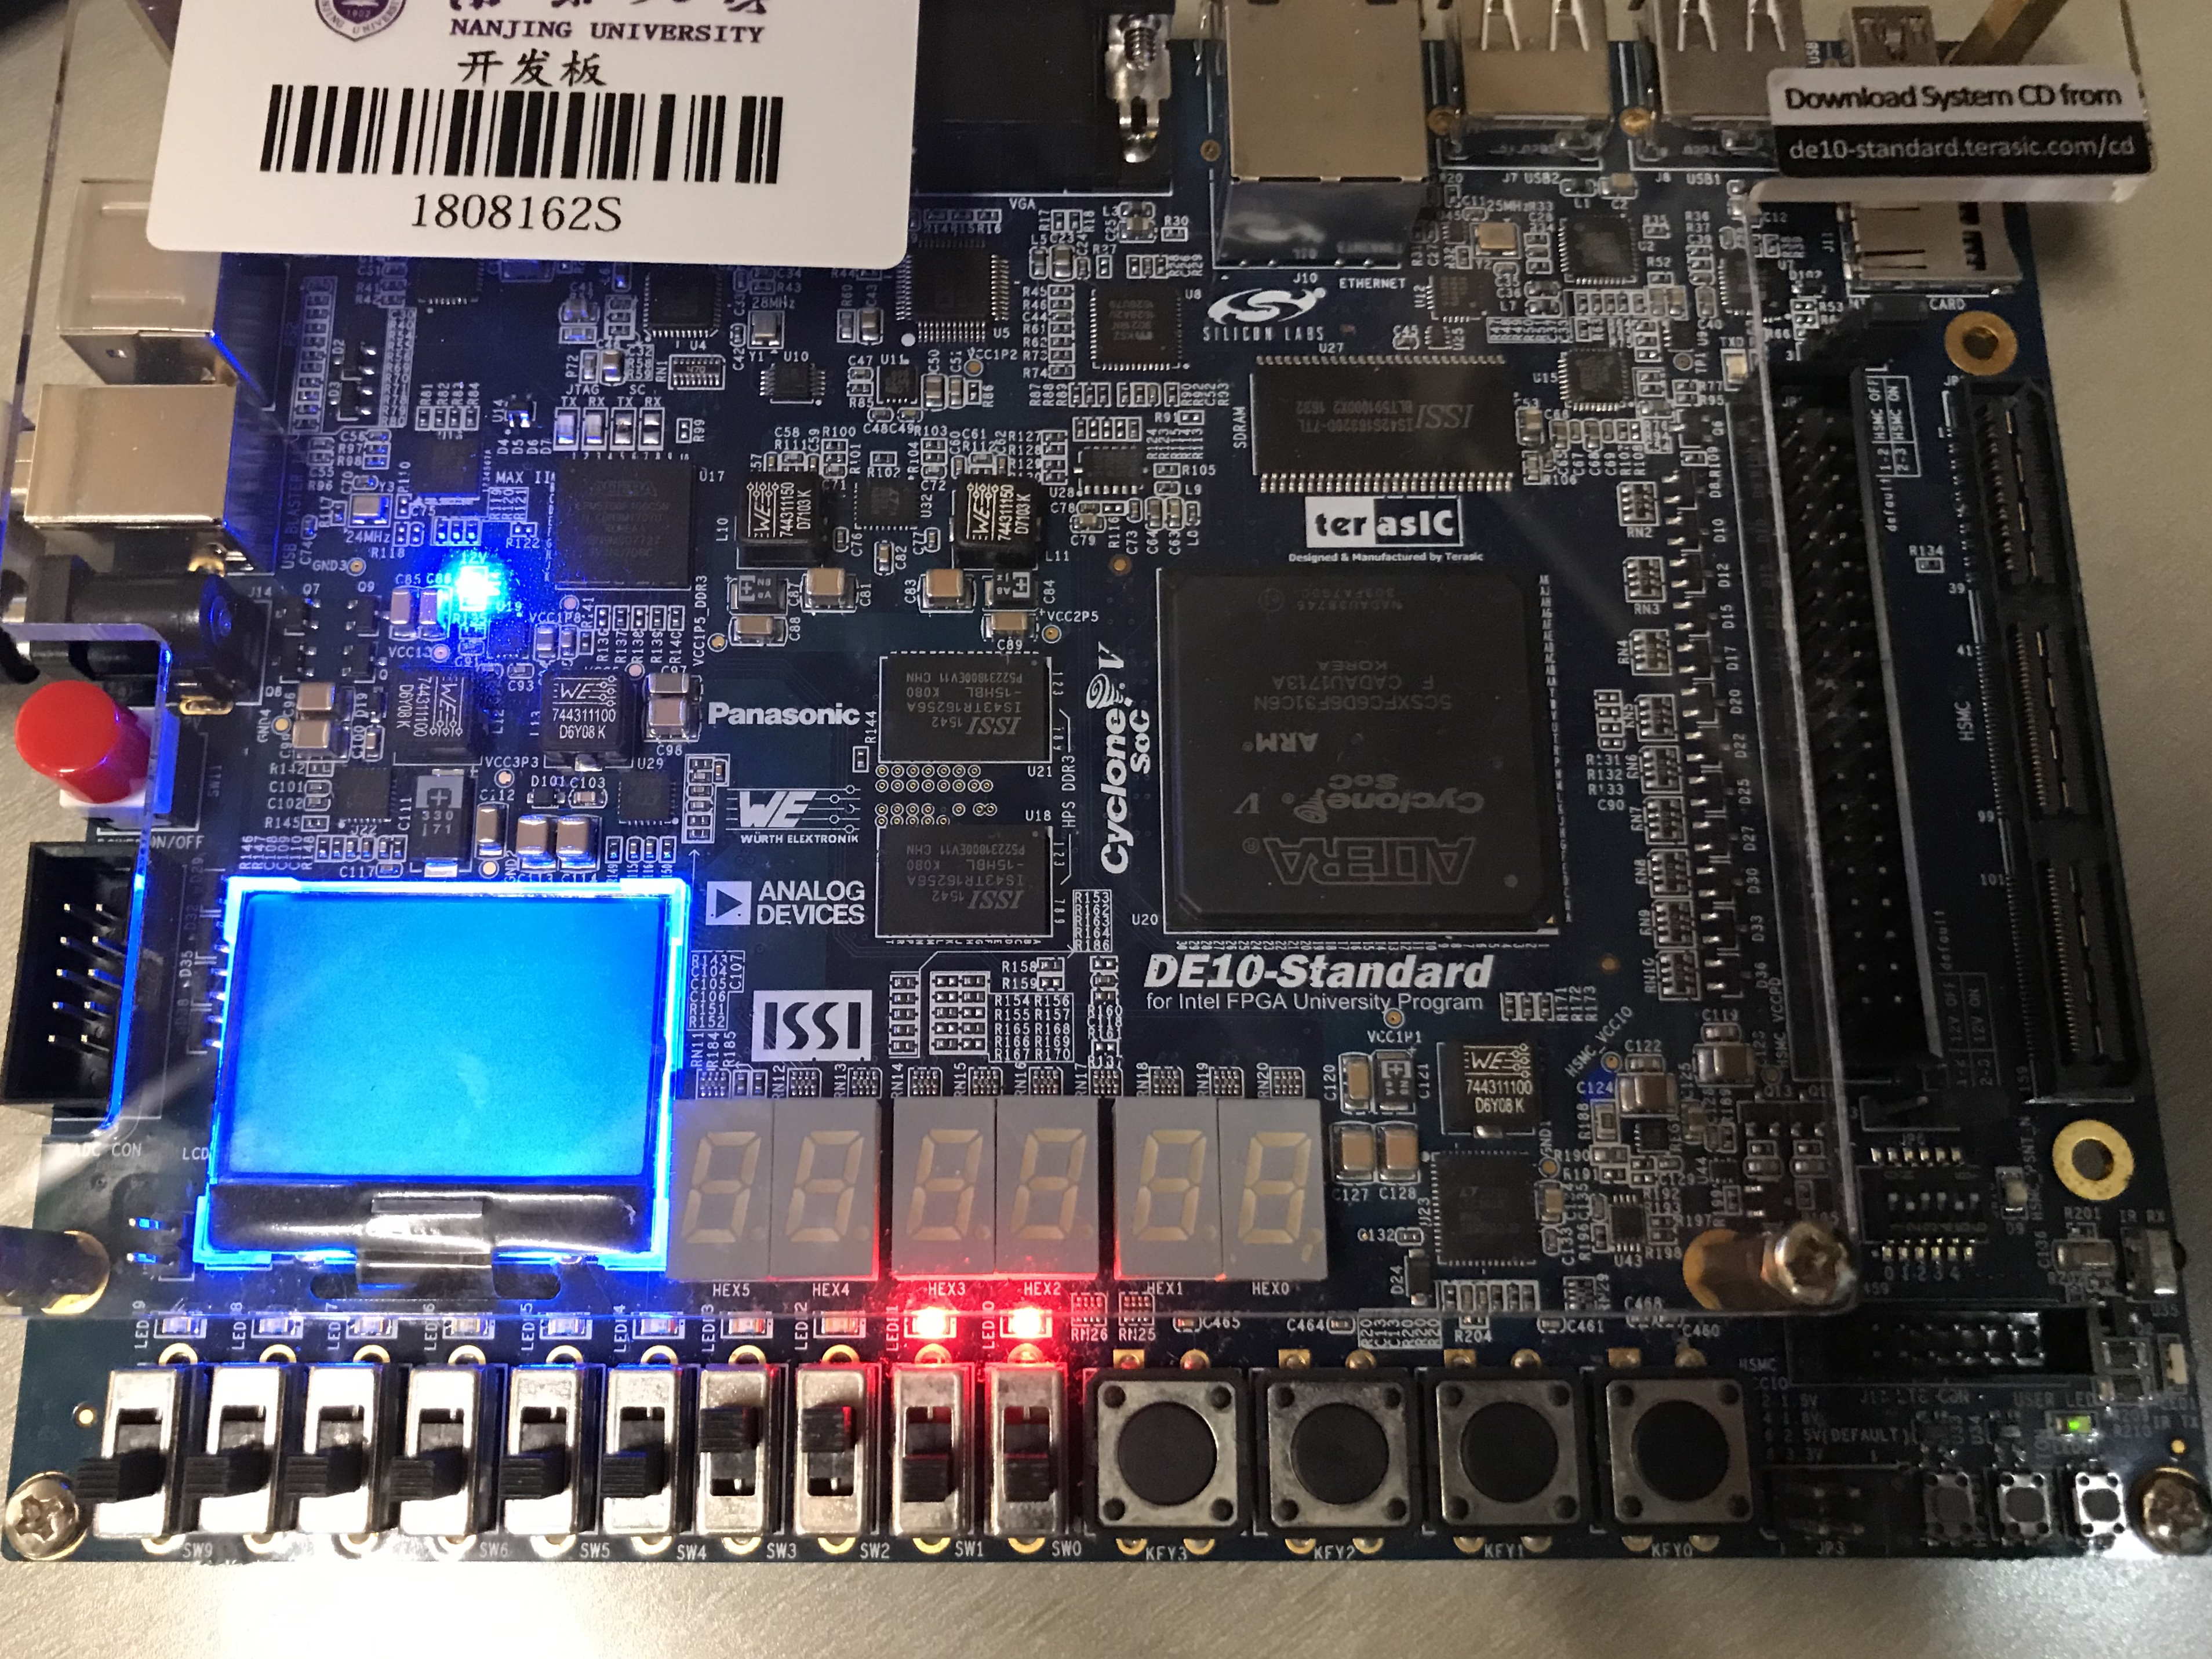
\includegraphics[width=0.45\textwidth]{fpga2.JPG}
  }
  \caption{FPGA验证}
  \label{fpga}
\end{figure}

做完之后才发现这题好像可以用case语句做……
懒得改了就这样吧反正效果一样的……下一题我再用case语句做

\subsection{实验2.3 8-3优先编码器}
\begin{itemize}
  \item 这题还是很简单的一道题,先进行优先编码,然后译码到七段数码管上
  \item 优先编码的代码中用了disable语句,可以在找到第一个有效位之后直接跳出循环
  \item 我把优先编码器的输入指示位放在了输出LEDR的最低位,所以在七段译码器的case语句中,
        数码管的输入(也就是优先编码器的输出LEDR)相当于左移之后再加1
        (因为如果有输入则指示位必定为1)
  \item 无有效输入的情况下(即8个开关全0时),七段数码管显示`8'
\end{itemize}
\begin{lstlisting}[style=verilog-style]
  begin : CODE
  Y[3:0] = 4'b0000;
  for (i = 7; i >= 0; i = i - 1)
    if (X[i] == 1) begin
      Y[3:1] = i;
      Y[0] = 1;
      disable CODE;
    end
  end
  case (Y)
    4'd1 : Z = 7'b1000000;
    4'd3 : Z = 7'b1111001;
    4'd5 : Z = 7'b0100100;
    4'd7 : Z = 7'b0110000;
    4'd9 : Z = 7'b0011001;
    4'd11 : Z = 7'b0010010;
    4'd13 : Z = 7'b0000010;
    4'd15 : Z = 7'b1111000;
    default : Z = 7'b0000000;
  endcase
\end{lstlisting}

用RTL Viewer看一下内部结构:
\begin{figure}[H]
  \centering
  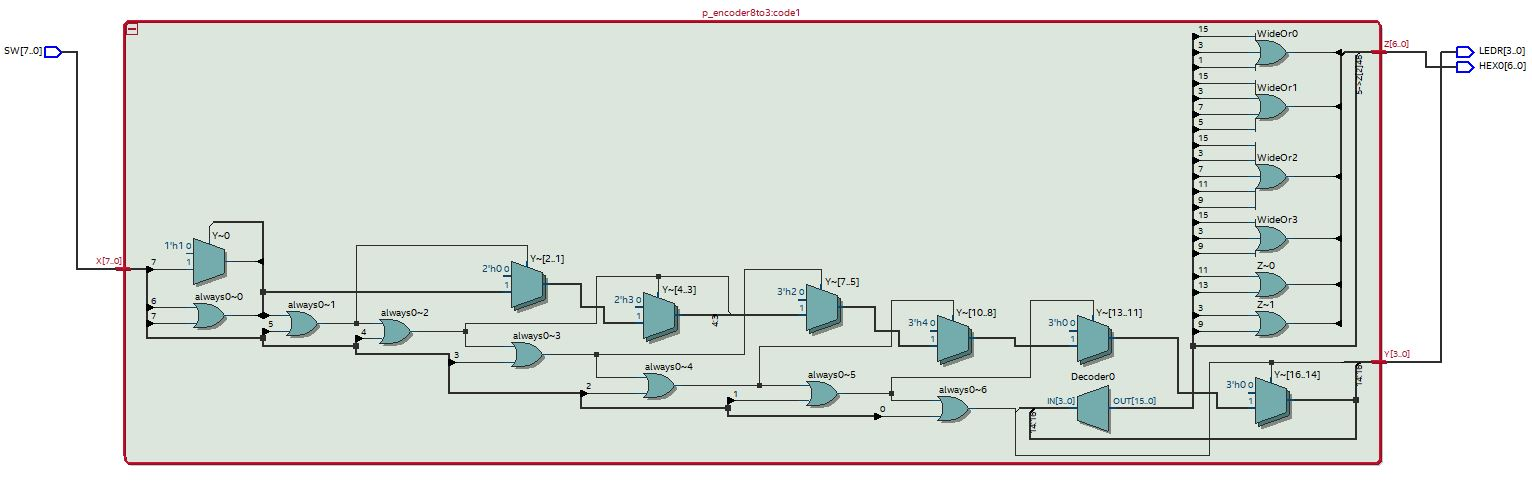
\includegraphics[width=0.8\textwidth]{2_3RTL.JPG}
  \caption{RTL Viewer}
  \label{8to3_RTL}
\end{figure}

运行仿真一下,上面7个是输入,中间4个是LEDR,下面七个是HEX0:
\begin{figure}[H]
  \centering
  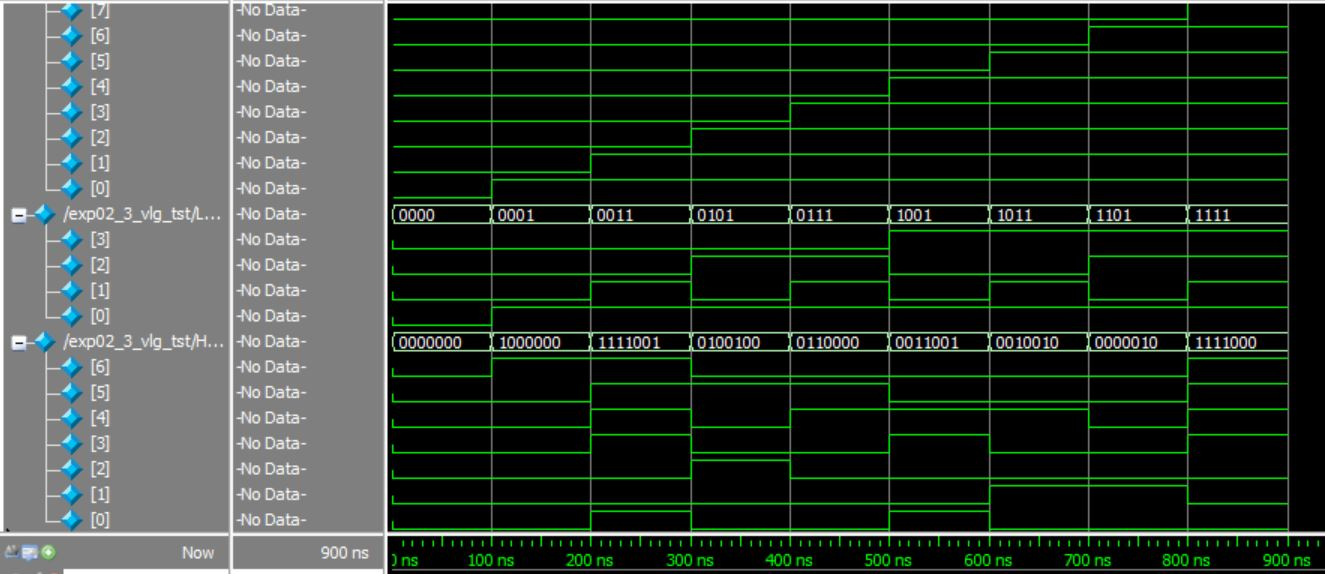
\includegraphics[width=0.8\textwidth]{2_3sim.JPG}
  \caption{仿真波形图}
  \label{8to3_sim}
\end{figure}

下载到FPGA开发板上验证,满足实验要求
\begin{figure}[H]
  \centering
  \subfigure{
    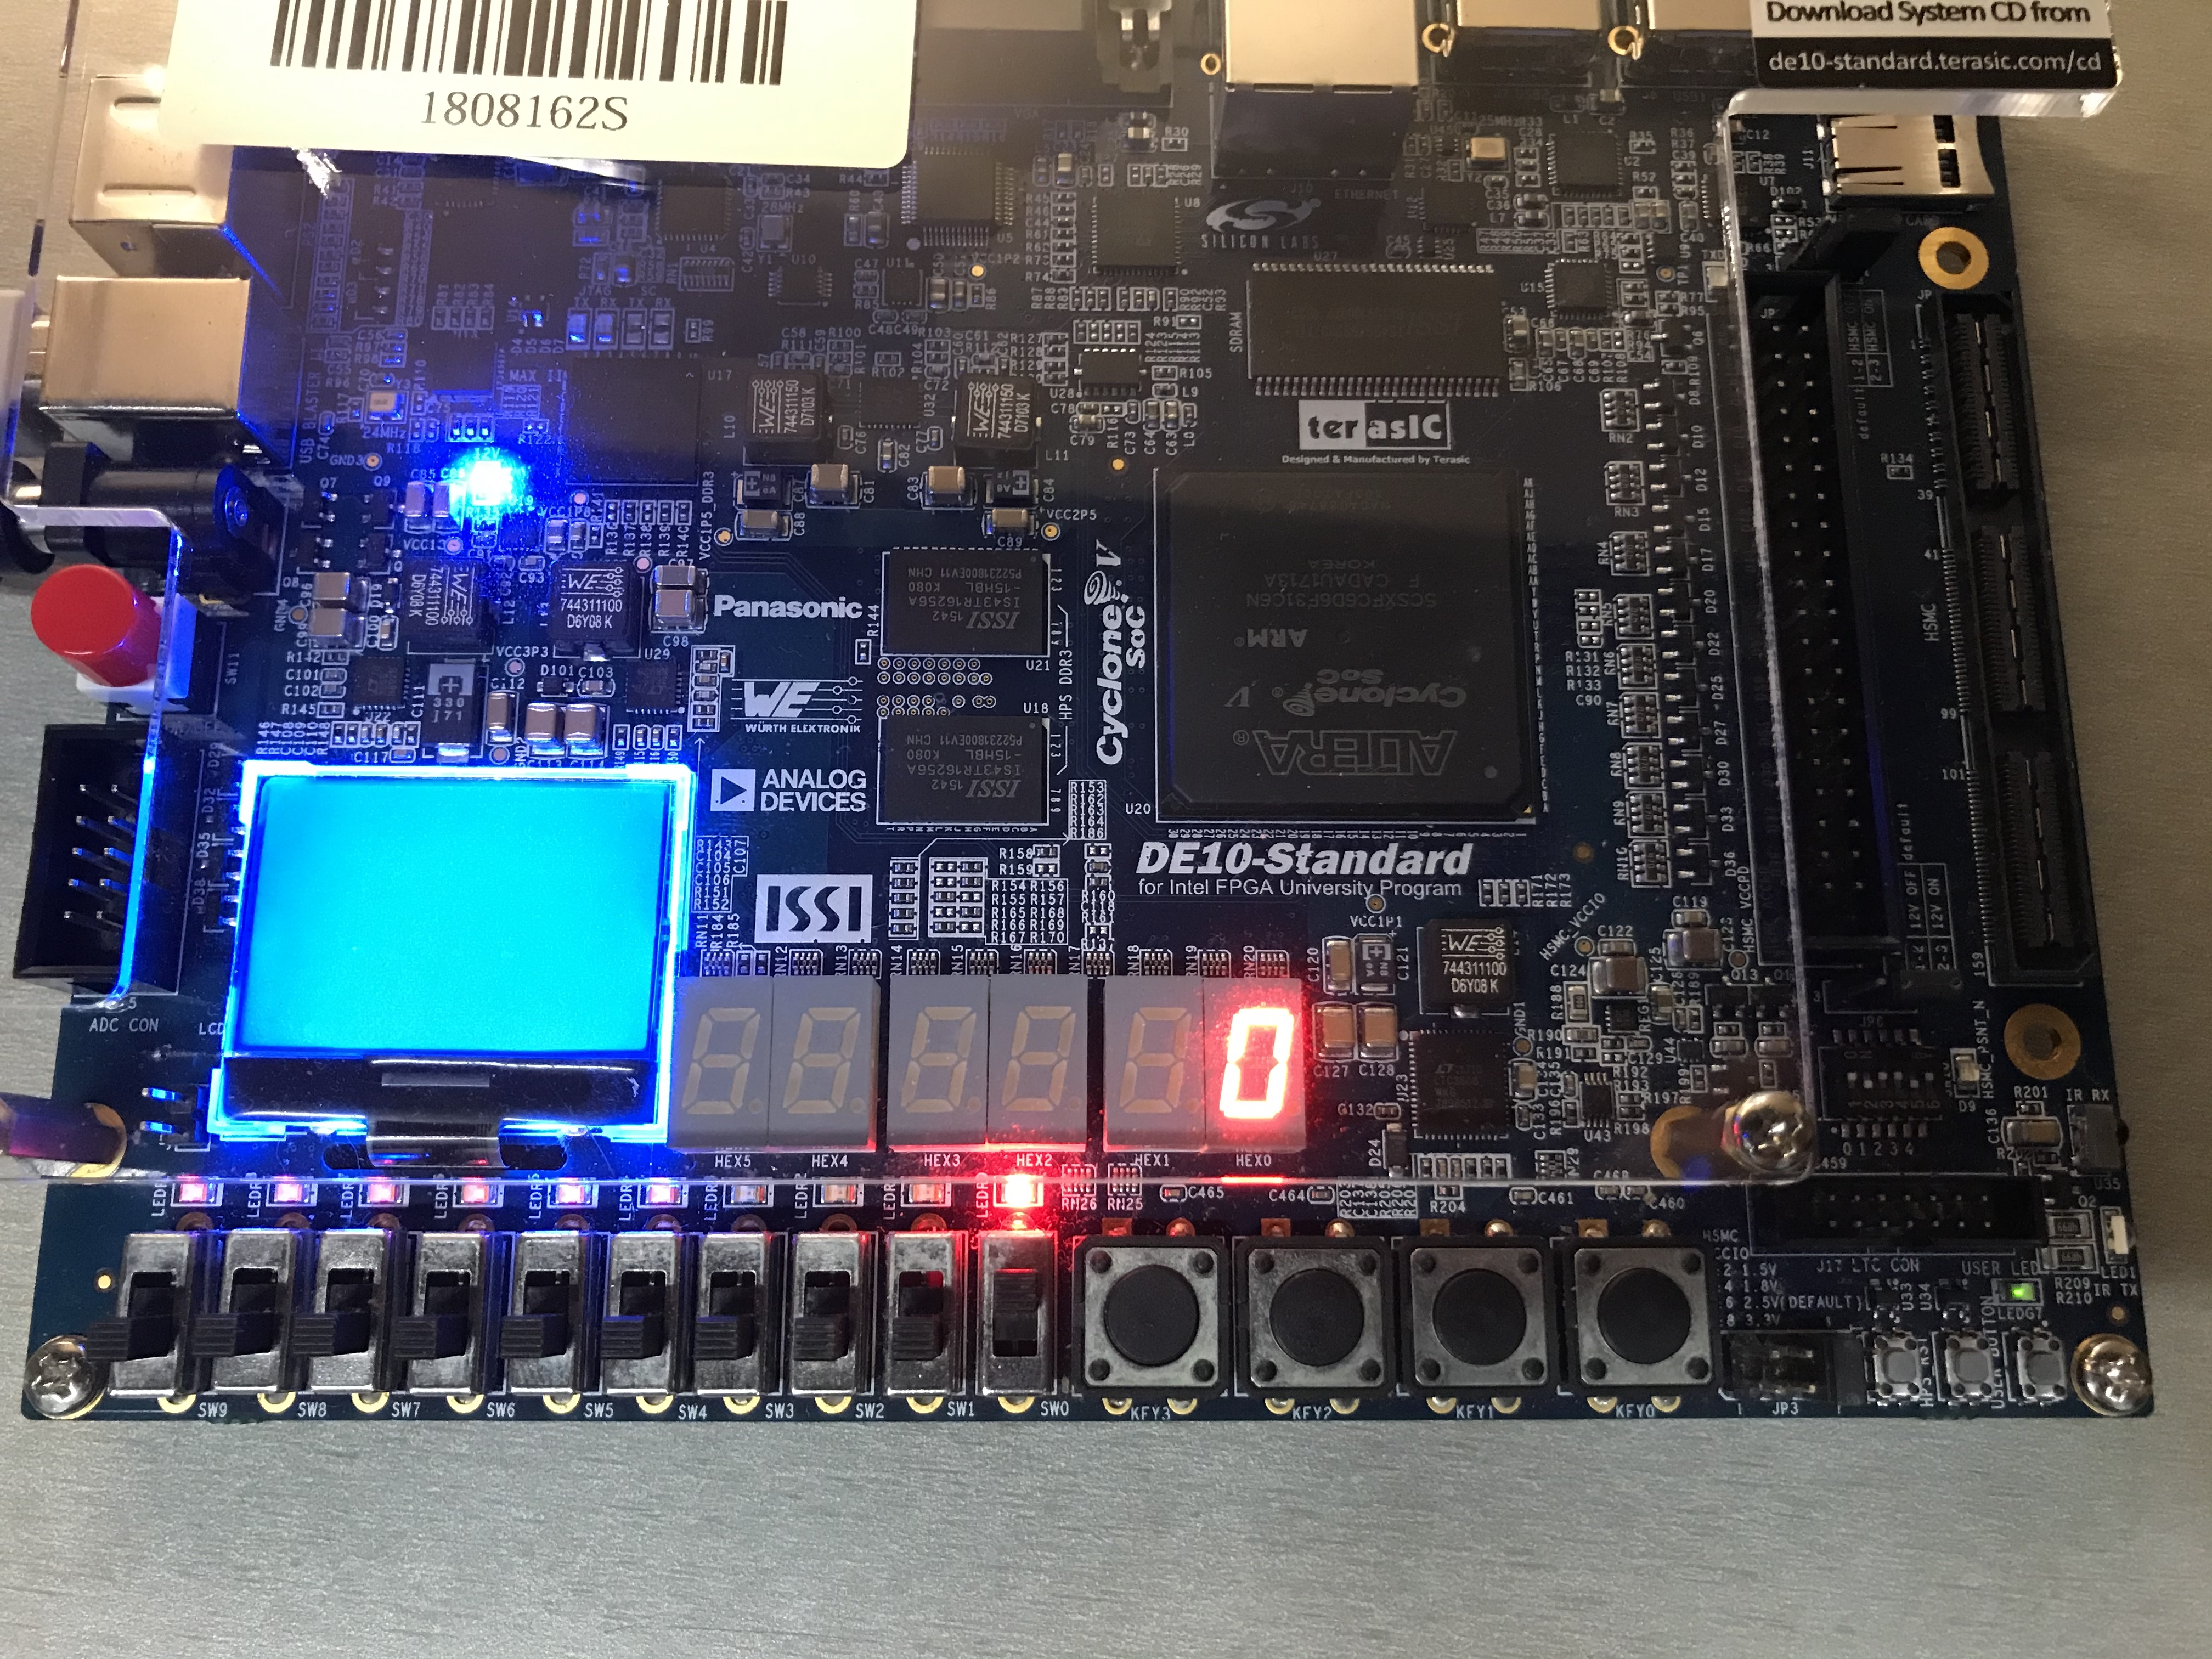
\includegraphics[width=0.45\textwidth]{fpga3.JPG}
  }
  \subfigure{
    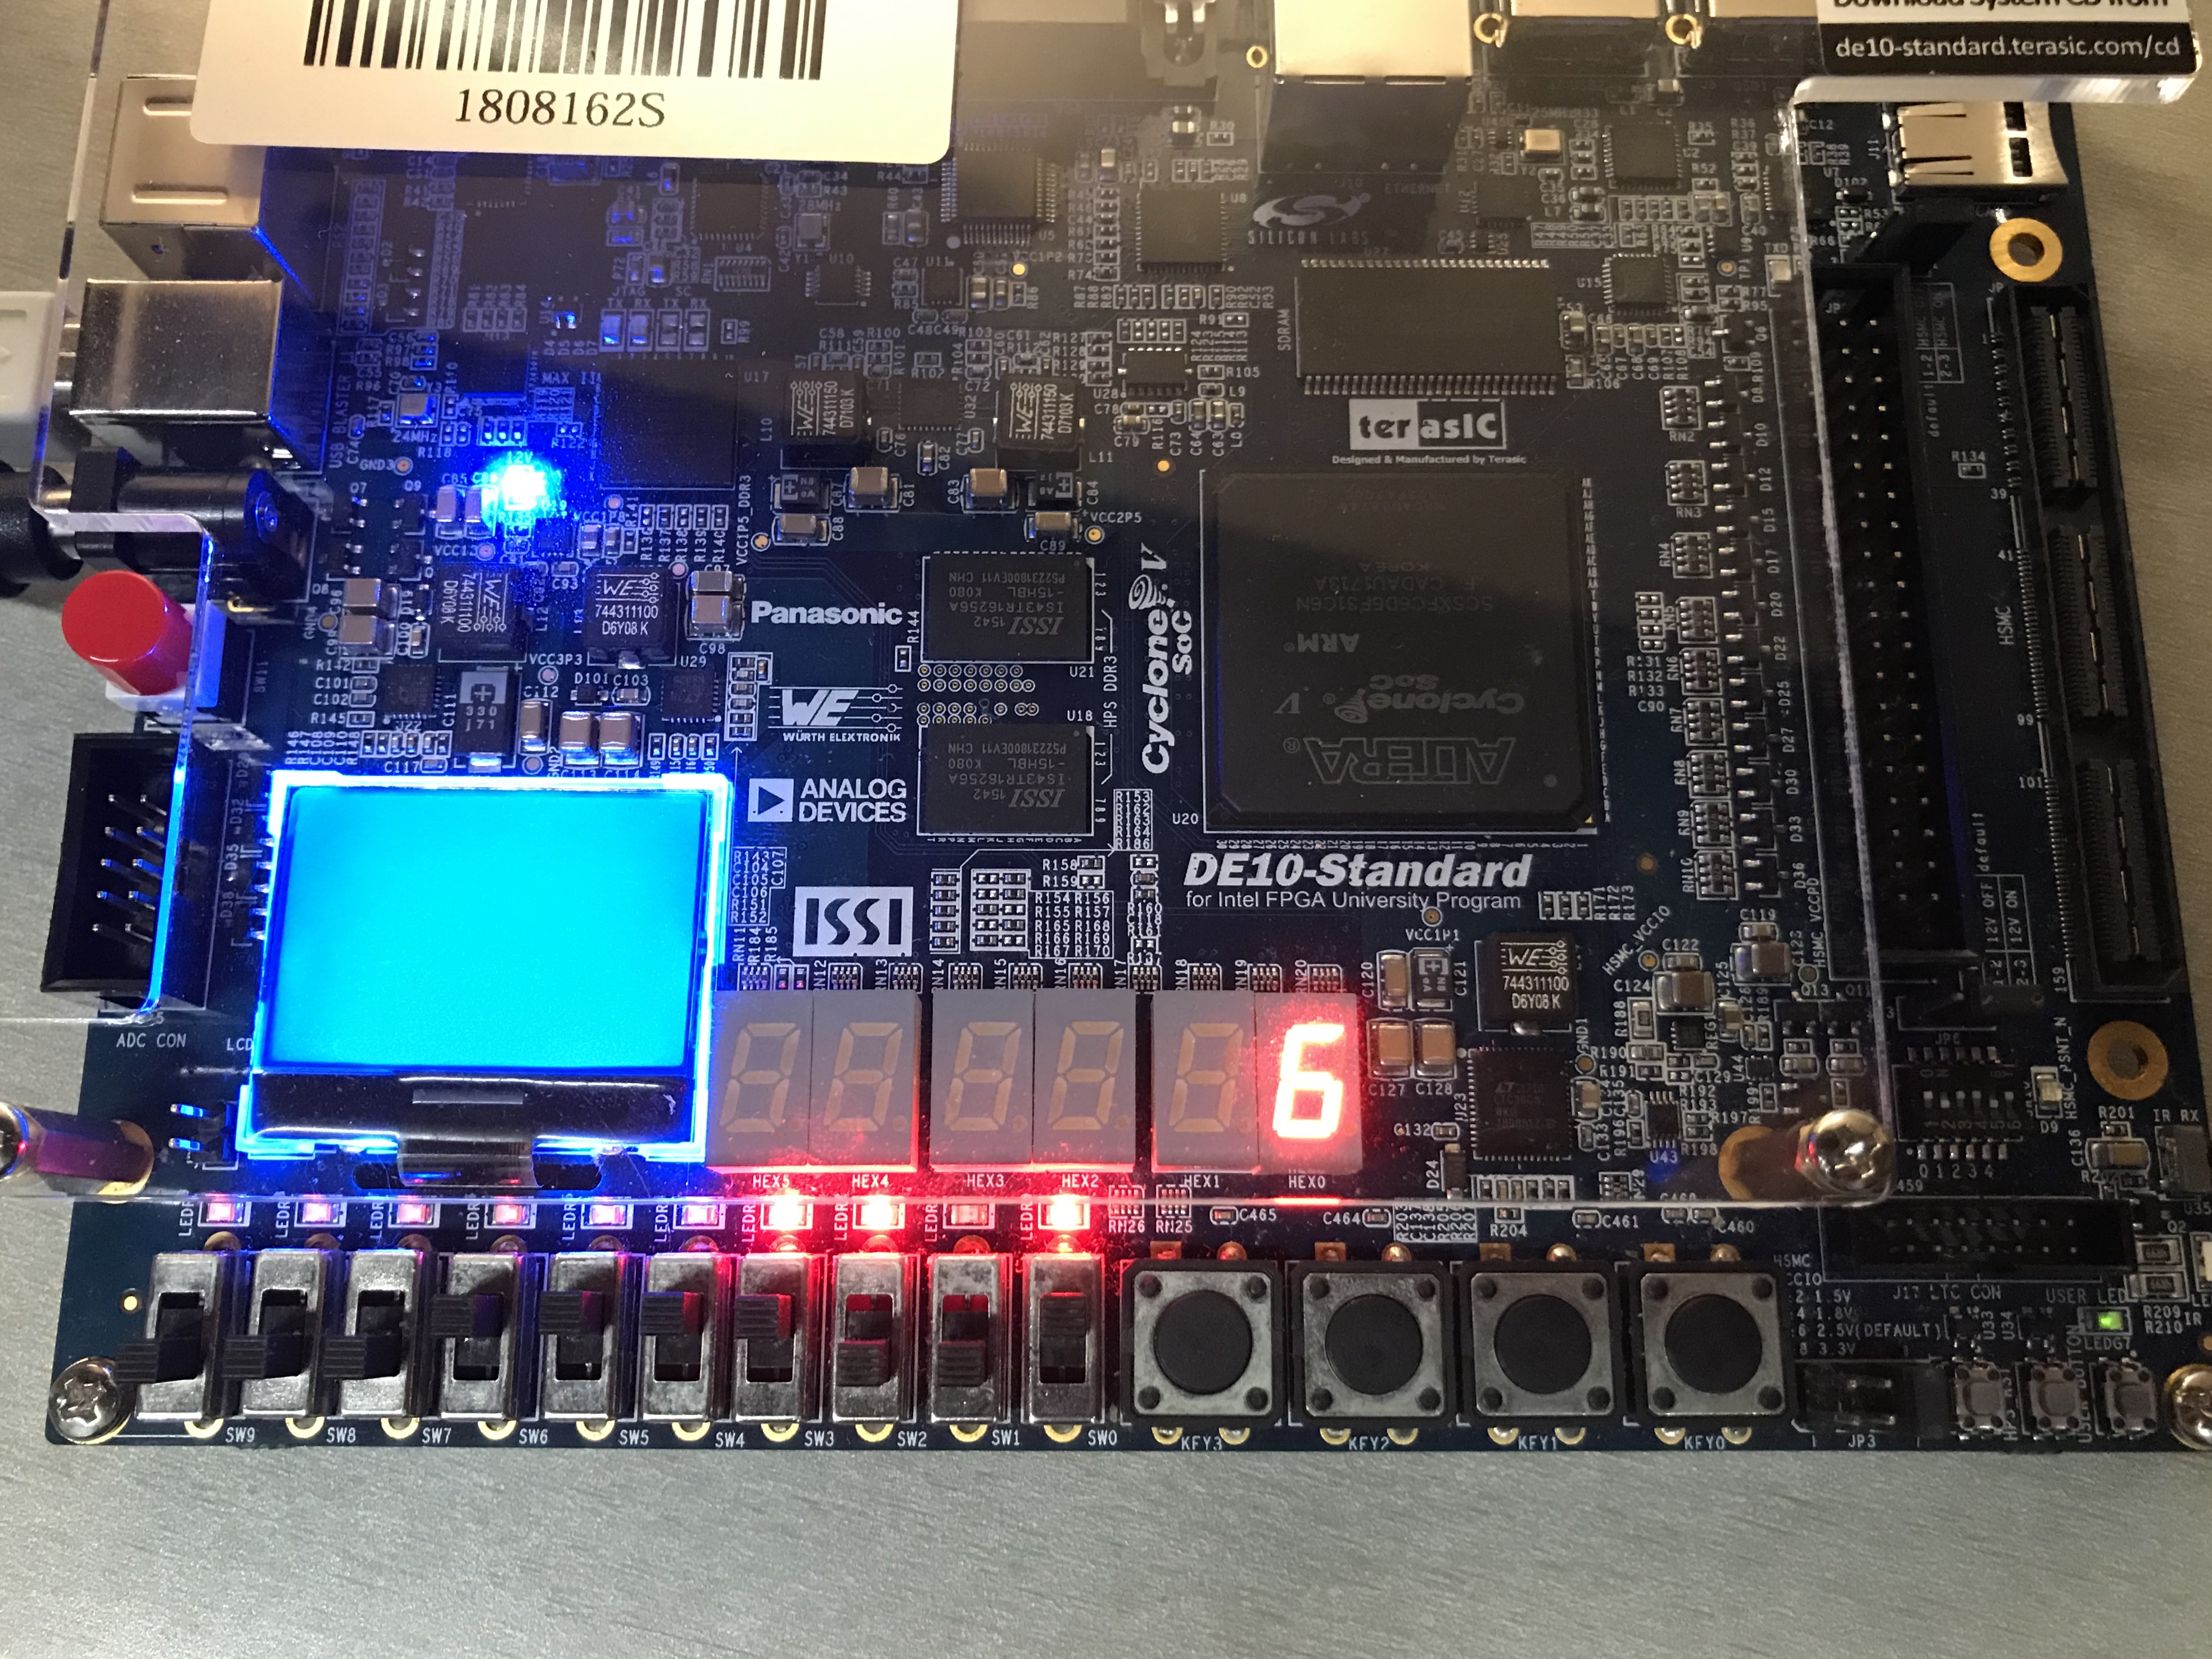
\includegraphics[width=0.45\textwidth]{fpga4.JPG}
  }
  \caption{FPGA验证}
  \label{fpga}
\end{figure}

\subsection{实验2.3 用casex语句设计优先编码器}
对于每个case n,其二进制值右数第n+1位为1,该位左边全是0,右边全是x
\begin{lstlisting}[style=verilog-style]
  casex (sel)
    8'b00000001 : Z = 7'b1000000;
    8'b0000001x : Z = 7'b1111001;
    8'b000001xx : Z = 7'b0100100;
    8'b00001xxx : Z = 7'b0110000;
    8'b0001xxxx : Z = 7'b0011001;
    8'b001xxxxx : Z = 7'b0010010;
    8'b01xxxxxx : Z = 7'b0000010;
    8'b1xxxxxxx : Z = 7'b1111000;
    default : Z = 7'b0000000;
  endcase
\end{lstlisting}

\section{实验结果}
\begin{itemize}
  \item 3个程序都在电脑上运行成功并且满足实验题目要求
  \item 分别用assign语句和case语句两种方法实现了七段译码器
        \sout{(要是我早一点想起来用case语句谁会去化简卡诺图写assign啊)}
  \item 在FPGA开发板上运行的实验2.2.3和实验2.3都成功了
\end{itemize}

\section{遇到的问题及解决办法}
\begin{itemize}
  \item 在实验2.2.3中,用DE10\_Standard\_SystemBuilder创建工程后,
        如果不修改主模块默认的输入输出的话,下载到FPGA之后空接的那几个七段数码管会亮
        (也就是HEX5$\sim$HEX1都会显示数字`8'),所以要将主模块的输入和输出
        修改为我们要用到的那几个引脚(这样做之后编译的时候警告也会少很多)
  \item 一开始写的case语句是对Y[3:1]进行选择对应到case0$\sim$7,
        后来发现全0输入和8'b00000001输入在七段数码管上都显示0,
        所以改为对Y进行选择,对应的case为0$\sim$15之间的奇数case
        (详见上文的实验代码)。这样全0输入时七段数码管会显示`8'
\end{itemize}

\section{得到的启示}
\begin{itemize}
  \item 实验2.2.2的代码效率有点低。该代码表示高位优先的优先级编码器,
        所以for循环应该从高位向低位递减,当遇到第一个高位为1时用disable语句跳出循环
        (所描述的方法已在实验2.3中实现)
  \item 实现七段译码器的方法是多种多样的\sout{(我已经不想再提卡诺图的事了)}
\end{itemize}

\section{意见和建议}
\begin{itemize}
  \item 希望可以在每个实验题目pdf的末尾描述一下需要提交哪些文件
\end{itemize}

\end{document}